\documentclass[10pt, a4paper]{article}

\usepackage[utf8]{inputenc}
\usepackage[english, spanish]{babel}
\usepackage[left=25mm, right=25mm, top=35mm, bottom=30mm, headheight=35mm]{geometry}
\usepackage{graphicx}
\usepackage{float}
\usepackage{xcolor}
\usepackage{fancyhdr}
\usepackage{hyperref}
\usepackage{setspace}
\usepackage{indentfirst}

% Syntax customization with minted package
\usepackage{minted}
\usepackage[outputdir=build]{minted}
\usemintedstyle{nord-darker}
\usemintedstyle[zsh]{gruvbox-light}
\setminted{
  breaklines,
  linenos,
  frame=lines,
  fontsize=\normalsize,
  bgcolor=background
}

% shoetcut to include python code in a line
\newcommand{\mpy}[1]{\mintinline[style=gruvbox-light]{python}{#1}}

% Define background color
\definecolor{background}{HTML}{2E3440}

% Variables
\newcommand{\university}{Universidad Nacional de San Agustín de Arequipa}
\newcommand{\faculty}{Facultad de Ingeniería de Producción y Servicios}
\newcommand{\program}{Escuela Profesional de Ingeniería de Sistemas}
\newcommand{\semester}{2024 - A}
\newcommand{\course}{img/web_programming.png}
\newcommand{\topic}{img/django_react.png}
\newcommand{\professor}{Carlo Jose Luis Corrales Delgado}
\newcommand{\students}{Yenaro Joel Noa Camino\\Armando Steven Cuno Cahuari\\Victor Narciso Mamani Anahua\\Jorge Luis Mamani Huarsaya}
\newcommand{\github}{https://github.com/ynoacamino/pweb2-final-project}
\newcommand{\figma}{https://www.figma.com/design/m7RQxtCLrHm5ZyCNtoCk6J/Learning-Plataform?node-id=0-1&t=Kgg9BpkP8D86LnTM-0}
\newcommand{\mydate}{6 de julio, 2024}

% Just parts and chapters numbered
\setcounter{secnumdepth}{0}

% Head and foot customization
\pagestyle{fancy}
\lhead{\raisebox{-0.2\height}{
\includegraphics[width=4cm]{img/logo_unsa.png}}}
\chead{\fontsize{8}{8}\selectfont \university \\ \faculty \\ \textbf{\program}}
\rhead{\raisebox{-0.2\height}{
\includegraphics[width=3.5cm]{img/logo_episunsa.png}}}
\lfoot{Semestre \semester}
\cfoot{}
\rfoot{Pág. \thepage}

\begin{document}

\begin{titlepage}
	\centering
	\includegraphics[width=15cm]{\course} \par
  \vfill \vfill
	\includegraphics[width=15cm]{\topic}\par
  \vfill \vfill
  {\textbf{Profesor(a):} \par}
	\professor \vfill
  {\textbf{Estudiantes:} \par}
	\students \vfill
  {\textbf{Repositorio GitHub:} \par}
  \href{\github}{\github} \vfill
  {\textbf{Link del Figma:} \par}
  \href{\figma}{\figma} \vfill
	{\large \mydate \par}
\end{titlepage}

\section*{Backend - Proyecto PWEB}
En esta sección, explicaremos detalladamente la implementación del backend para el proyecto.
\subsection*{Descripcion General}
El backend del proyecto está construido utilizando Django, un framework de alto nivel para el desarrollo de aplicaciones web en Python.
\subsection*{Estructura del Proyecto}
\begin{minted}[bgcolor=white]{text}
	server/
	│-- academia/
	│   │-- migrations/         # Archivos de migraciones de base de datos
	│   │   |-- __init__.py     # Inicialización del módulo de migraciones
	│   │   |-- 0001_initial.py # Migración inicial
	│   │-- __init__.py         # Inicialización del módulo academia
	│   │-- admin.py            # Registro de modelos en el admin de Django
	│   │-- apps.py             # Configuración de la aplicación academia
	│   │-- models.py           # Definición de modelos de datos
	│   │-- serializers.py      # Serializadores para la API
	│   │-- tests.py            # Pruebas unitarias para la aplicación
	│   │-- urls.py             # Enrutamiento de URLs específicas de la aplicación
	│   │-- views.py            # Vistas y lógica de controladores
	│-- media_manager/
	│   │-- migrations/         # Archivos de migraciones de base de datos
	│   │   |-- __init__.py     # Inicialización del módulo de migraciones
	│   │-- __init__.py         # Inicialización del módulo media_manager
	│   │-- admin.py            # Registro de modelos en el admin de Django
	│   │-- apps.py             # Configuración de la aplicación media_manager
	│   │-- urls.py             # Enrutamiento de URLs específicas de la aplicación
	│   │-- views.py            # Vistas y lógica de controladores
	│-- server/
	│   │-- __init__.py         # Inicialización del módulo principal del proyecto
	│   │-- asgi.py             # Configuración para el servidor ASGI
	│   │-- settings.py         # Configuraciones del proyecto Django
	│   │-- urls.py             # Enrutamiento de URLs del proyecto principal
	│   │-- wsgi.py             # Configuración para el servidor WSGI
	│-- .env.example            # Archivo de ejemplo para las variables de entorno
	│-- db.sqlite3              # Archivo de base de datos SQLite (para desarrollo)
	│-- manage.py               # Script principal para gestionar el proyecto
	│-- requirements.txt        # Lista de dependencias del proyecto
\end{minted}
La estructura del proyecto está diseñada para facilitar la organización, el mantenimiento y la escalabilidad. A continuación, se presentará dicha estructura.
\subsection*{Flujo de Trabajo}
\begin{enumerate}
	\item El usuario enviara una solicitud HTTP al servidor.
	\item La solicitud se enrutara atraves de los archivos 'urls.py' al controlador adecuado en el modulo de vistas.
	\item El controlador maneja la logica de la solicitud, interactua con los modelos de datos y utiliza los serializadores si es necesario.
	\item La respuesta es devuelta al usuario en formato JSON atraves de la API RESTful
\end{enumerate}
Explicaremos la composición de cada módulo en nuestro proyecto para ilustrar el flujo de trabajo de Django utilizado para el backend.
\subsection*{Módulo Academia}
La creación de nuestra aplicación dentro del proyecto backend es fundamental ya que cumple roles esenciales. Cada aplicación en Django actúa como un componente independiente que gestiona una parte específica de la funcionalidad del proyecto. 
\begin{enumerate}
	\item \textbf{Módulo models}: \\
	Definiremos varios modelos en Django para el proyecto relacionado con cursos, usuarios, reseñas, PDFs, entre otros. Cada modelo utilizará diferentes tipos de campos para su representación en la base de datos. Estableceremos relaciones entre estos modelos utilizando `ManyToManyField` y `ForeignKey` según sea necesario para capturar las interacciones y la estructura de datos requerida por la aplicación.
	Las relaciones que guardan los modelos son:\\
	Relacion de uno a muchos:
	\begin{itemize}
		\item Curso a Teacher
		\item Review a User
		\item Review a Curso
		\item Section a Curso
		\item Pdf a Section
	\end{itemize}
	Relacion de muchos a muchos:
	\begin{itemize}
		\item Curso a User
	\end{itemize}
	\begin{minted}{python}
		from django.db import models
		
		class Teacher(models.Model):
		teacher_id = models.IntegerField(primary_key=True)
		name = models.CharField(max_length=255)
		phone_number = models.CharField(max_length=255)
		email = models.EmailField()
		
		def _str_(self):
		return self.name
		
		class User(models.Model):
		user_id = models.IntegerField(primary_key=True)
		name = models.CharField(max_length=255)
		phone_number = models.CharField(max_length=255)
		email = models.EmailField()
		
		def _str_(self):
		return self.name
		
		class Curso(models.Model):
		curso_id = models.IntegerField(primary_key=True)
		name = models.CharField(max_length=255)
		description = models.TextField()
		teacher = models.ForeignKey(Teacher, on_delete=models.CASCADE)
		users = models.ManyToManyField(User, related_name='usuarios')
		
		def _str_(self):
		return self.name
		
		class Review(models.Model):
		comment = models.TextField()
		user = models.ForeignKey(User, on_delete=models.CASCADE)
		curso = models.ForeignKey(Curso, on_delete=models.CASCADE)
		
		def _str_(self):
		return f'Reseña hecho/a por {self.user.name} hacia el curso {self.curso.name}'
		
		class Section(models.Model):
		section_id = models.IntegerField(primary_key=True)
		curso = models.ForeignKey(Curso, on_delete=models.CASCADE)
		name = models.CharField(max_length=255)
		description = models.TextField()
		video_url = models.URLField(max_length=200)
		
		def _str_(self):
		return self.name
		
		class Pdf(models.Model):
		name = models.CharField(max_length=255)
		url = models.URLField(max_length=200)
		section = models.ForeignKey(Section, on_delete=models.CASCADE)
		
		def _str_(self):
		return self.name
	\end{minted}
	\item \textbf{Módulo admin}: \\
	Será necesario registrar los modelos definidos en el proyecto para que puedan ser gestionados a través del panel de administración de Django. Utilizaremos `admin.site.register` para registrar estos modelos, lo que facilitará la gestión y el mantenimiento del sistema al permitirnos administrar y modificar los datos de manera eficiente desde la interfaz de administración de Django.
	\begin{minted}{python}
		from django.contrib import admin
		from .models import *
		
		admin.site.register(Teacher)
		admin.site.register(User)
		admin.site.register(Curso)
		admin.site.register(Review)
		admin.site.register(Section)
		admin.site.register(Pdf)
	\end{minted}
	\item \textbf{Módulo apps}: \\
	La función de este módulo será configurar la aplicación y proporcionar metadatos sobre ella para que Django la reconozca y gestione correctamente. Para lograr esto, implementaremos una clase `AcademiaConfig` que contendrá las configuraciones específicas de la aplicación. Esta clase incluirá información necesaria para referirse y gestionar la aplicación dentro del entorno de Django, como el nombre de la aplicación y configuraciones adicionales que puedan ser requeridas, como configuraciones de permisos o configuraciones de visualización en el panel de administración.
	\begin{minted}{python}
		from django.apps import AppConfig
		
		class AcademiaConfig(AppConfig):
		default_auto_field = 'django.db.models.BigAutoField'
		name = 'academia'	
	\end{minted}
	\item \textbf{Módulo serializers}: \\
	Para emplear Django REST Framework, es necesario definir este módulo. Los serializadores en DRF se encargan de convertir objetos de Django en formatos de datos manipulables, como JSON. Esto es crucial para aplicaciones web donde la transferencia eficiente de datos entre el frontend y el backend es fundamental. Implementaremos un serializador para cada modelo necesario, cada uno recopilando la información del modelo correspondiente. Además, utilizaremos la clase `Meta` en cada serializador para especificar el modelo y los campos que se deben serializar. Esto asegura que los datos sean presentados de manera coherente y eficiente para su manipulación en la aplicación.
	\begin{minted}{python}
		from rest_framework import serializers
		from .models import *
		
		class TeacherSerializer(serializers.ModelSerializer):
		class Meta:
		model = Teacher
		fields = ['teacher_id', 'name', 'phone_number', 'email']
		
		class UserSerializer(serializers.ModelSerializer):
		class Meta:
		model = User
		fields = ['user_id', 'name', 'phone_number', 'email']
		
		class CursoSerializer(serializers.ModelSerializer):
		class Meta:
		model = Curso
		fields = ['curso_id', 'name', 'description', 'teacher', 'users']
		
		class ReviewSerializer(serializers.ModelSerializer):
		class Meta:
		model = Review
		fields = ['comment', 'user', 'curso']
		
		class SectionSerializer(serializers.ModelSerializer):
		class Meta:
		model = Section
		fields = ['section_id', 'curso', 'name', 'description', 'video_url']
		
		class PdfSerializer(serializers.ModelSerializer):
		class Meta:
		model = Pdf
		fields = ['name', 'url', 'section']	
	\end{minted}
	\item \textbf{Módulo urls}: \\
	Para emplear Django REST Framework y configurar las URLs de la API, utilizaremos el enrutador `DefaultRouter`. Este enrutador nos permite gestionar las rutas de la API basadas en las vistas `ViewSet` de manera automática. Aquí está cómo lo haremos:
	\begin{itemize}
		\item Crearemos una instancia de `DefaultRouter`.
		\item Registraremos cada `ViewSet` en el enrutador para que genere automáticamente las rutas correspondientes.
	\end{itemize}
	Esto simplifica significativamente el proceso de definición y mantenimiento de las rutas de la API dentro de nuestra aplicación, asegurando que las URL se gestionen de manera coherente y eficiente.
	\begin{minted}{python}
		from rest_framework import routers
		from .views import *
		
		router = routers.DefaultRouter()
		
		router.register('api/user', UserViewSet, 'user')
		router.register('api/teacher', TeacherViewSet, 'teacher')
		router.register('api/curso', CursoViewSet, 'curso')
		router.register('api/review', ReviewViewSet, 'review')
		router.register('api/section', SectionViewSet, 'section')
		router.register('api/pdf', PdfViewSet, 'pdf')
		
		urlpatterns = router.urls	
	\end{minted}
	\item \textbf{Módulo views}: \\
	Para emplear Django REST Framework y gestionar las operaciones CRUD en los modelos de la base de datos, utilizaremos un conjunto de vistas (`ViewSet`). Cada `ViewSet` estará encargado de manejar las solicitudes HTTP, interactuar con la base de datos y presentar los datos correspondientes. Aquí está cómo lo haremos:
	
	\begin{itemize}
		\item \textbf{Definición del ViewSet} \\
		Crearemos un ViewSet para cada modelo que necesitemos manejar. Este ViewSet contendrá métodos para realizar operaciones CRUD (Create, Retrieve, Update, Delete).
		\item \textbf{Uso del serializador}\\
		Indicaremos y utilizaremos el serializador correspondiente para cada instancia del modelo dentro del ViewSet. El serializador se encargará de convertir los objetos de Django en formato de datos manipulable, como JSON, para las respuestas de la API.
		\item \textbf{Autenticacion y permisos} \\
		Configuraremos el ViewSet para que no requiera autenticación ni permisos especiales para acceder a las operaciones CRUD. Esto se hace configurando adecuadamente las clases de autenticación y permisos en la vista.	
	\end{itemize}
	Este enfoque nos permite manejar de manera eficiente las operaciones sobre los modelos de la base de datos a través de una API RESTful, asegurando que los datos sean presentados y manipulados de manera segura y coherente.
	\begin{minted}{python}
		from django.shortcuts import render
		from rest_framework import viewsets, permissions
		from .models import *
		from .serializers import *
		
		class UserViewSet(viewsets.ModelViewSet):
		queryset = User.objects.all()
		serializer_class = UserSerializer
		permission_classes = [permissions.AllowAny]
		
		class TeacherViewSet(viewsets.ModelViewSet):
		queryset = Teacher.objects.all()
		serializer_class = TeacherSerializer
		permission_classes = [permissions.AllowAny]
		
		class CursoViewSet(viewsets.ModelViewSet):
		queryset = Curso.objects.all()
		serializer_class = CursoSerializer
		permission_classes = [permissions.AllowAny]
		
		class ReviewViewSet(viewsets.ModelViewSet):
		queryset = Review.objects.all()
		authentication_classes = [permissions.IsAuthenticated]
		serializer_class = ReviewSerializer
		
		class SectionViewSet(viewsets.ModelViewSet):
		queryset = Section.objects.all()
		serializer_class = SectionSerializer
		permission_classes = [permissions.AllowAny]
		
		class PdfViewSet(viewsets.ModelViewSet):
		queryset = Pdf.objects.all()
		serializer_class = PdfSerializer
		permission_classes = [permissions.AllowAny]	
	\end{minted}
\end{enumerate}
\subsection*{Módulo Server}
En nuestro proyecto de Django, será necesario ajustar las configuraciones para definir el comportamiento y la funcionalidad de la aplicación de manera óptima. Esto incluye la configuración de aspectos como la base de datos, la autenticación, las rutas de la API, y otros parámetros importantes que afectan cómo se ejecuta y se comporta la aplicación.
\begin{enumerate}
	\item \textbf{Módulo settings}: \\
	Las configuraciones que establezcamos para el backend son esenciales para definir el comportamiento y la funcionalidad de nuestra aplicación.
	\begin{itemize}
		\item Será necesario definir las aplicaciones instaladas para que sean reconocidas por el proyecto. Esto incluye tanto las aplicaciones propias del proyecto como las dependencias externas, como Django REST Framework y sus extensiones.
		\begin{minted}{python}
			INSTALLED_APPS = [
			'media_manager',
			'academia',
			'django_extensions',
			'rest_framework',
			...
			]
		\end{minted}
		\item La base de datos que utiliza el proyecto de manera predeterminada en Django es SQLite. Esta base de datos es adecuada para el desarrollo y pruebas debido a su configuración simple y su facilidad de uso.
		\begin{minted}{python}
			DATABASES = {
				'default': {
					'ENGINE': 'django.db.backends.sqlite3',
					'NAME': BASE_DIR / 'db.sqlite3',
				}
			}
		\end{minted}	
	\end{itemize}
	\item \textbf{Modulo urls}: \\ 
	En este archivo definiremos la configuración de las URLs del proyecto Django. Esto especificará las rutas principales del proyecto y cómo se deben enrutar las solicitudes a las aplicaciones correspondientes. Al organizar las URLs de esta manera, mantenemos la configuración modular y manejable, lo que facilita el mantenimiento y la escalabilidad del proyecto.
	\begin{minted}{python}
		urlpatterns = [
		path('admin/', admin.site.urls),
		path('media_manager/', include('media_manager.urls')),
		path('academia/', include('academia.urls')),
		]
	\end{minted}
\end{enumerate}
\subsection*{Módulo Media-Manager}
Se desarrollará una aplicación dedicada al manejo de archivos multimedia, con la capacidad de gestionar la subida, almacenamiento y organización de estos archivos hacia la plataforma de Cloudinary. Esta integración asegurará que el proyecto maneje de manera eficiente los recursos multimedia, facilitando la gestión y optimización de los activos multimedia utilizados en la aplicación.
\begin{enumerate}
	\item \textbf{Modulo apps}: \\
	La clase `MediaManagerConfig` definirá la configuración específica de la aplicación, incluyendo cómo se manejan los campos y el nombre de la aplicación. Está diseñada para inicializar y gestionar adecuadamente estos aspectos dentro del entorno de Django.
	\begin{minted}{python}
		class MediaManagerConfig(AppConfig):
		default_auto_field = 'django.db.models.BigAutoField'
		name = 'media_manager'
	\end{minted}	
	\item \textbf{Modulo urls}: \\
	En este caso, la configuración de URLs apuntará directamente a una vista que ejecutará la función upload-route para manejar la solicitud y devolver la respuesta correspondiente. Aquí te muestro cómo podrías estructurar esto en el archivo urls.py de tu aplicación multimedia:
	\begin{minted}{python}
		urlpatterns = [
		path('upload/', upload_route, name='upload')
		]
	\end{minted}
	\item \textbf{Modulo views}: \\
	En esta vista de Django estara encargado de manejar la carga de archivos usando Cloudinary. 
	\begin{itemize}
		\item Para comenzar con la configuración necesaria en Django para manejar la subida de archivos multimedia y la integración con servicios como Cloudinary, necesitaremos realizar algunas importaciones y configuraciones clave. 
		\begin{itemize}
			\item \textbf{from django.http import HttpResponse:} Importa HttpResponse de django.http, que se utiliza para devolver respuestas HTTP desde la vista.
			\item \textbf{from dotenv import load-dotenv:} Importa load-dotenv de dotenv, que se usa para cargar variables de entorno desde un archivo .env.
			\item \textbf{load-dotenv():} Llama a la función load-dotenv() para cargar las variables de entorno definidas en un archivo .env. Esto es útil para manejar configuraciones sensibles como claves de API de Cloudinary de manera segura.
		\end{itemize}
		\begin{minted}{python}
			from django.http import HttpResponse
			
			from dotenv import load_dotenv
			load_dotenv()
		\end{minted}
		\item Después configuraremos adecuadamente Cloudinary. Para esto, es necesario importar la biblioteca de Cloudinary y especificar que se debe utilizar una conexión segura para todas las operaciones relacionadas con el almacenamiento y gestión de archivos multimedia.
		\begin{minted}{python}
			import cloudinary
			import cloudinary.uploader
			
			import json
			config = cloudinary.config(secure=True)
		\end{minted}
		\item Ahora, a través de una funcion llamada `uploadRoute`, nos encargaremos de manejar las solicitudes POST que llegan a la URL definida para la subida de archivos.
		\begin{itemize}
			\item Primero verificara si la solicitud es POST
			\item Luego extraera el archivo enviado en la solicitud POST desde request.FILES esperando los nombres del campo.
			\item Llamaremos a la funcion uploadFile con el archivo extraido y devuela la respuesta que esta funcion genera.
			\item Si la solicitud no es POST, devuelve una respuesta HTTP con el mensaje "Only post method allowed".
		\end{itemize}
		\begin{minted}{python}
			def upload_route(request):
			if request.method == 'POST':
			file = request.FILES['file']
			return uploadFile(file)
			return HttpResponse("Only post method allowed")
		\end{minted}
		\item Luego, mediante la función llamada `uploadFile`, se procede a cargar los archivos multimedia utilizando la API de Cloudinary. \\
		Primero, esta función cargará el archivo `file` a Cloudinary como un recurso automático. Luego, devolverá un diccionario con los datos de la carga. Finalmente, la función responderá con una respuesta HTTP que contiene estos datos de carga serializados en formato JSON.
		\begin{minted}{python}
			def uploadFile(file):
			upload_data = cloudinary.uploader.upload(file, resource_type = "auto")
			return HttpResponse(json.dumps(upload_data))
		\end{minted}
	\end{itemize}			
\end{enumerate}
\section{Los Componentes de la aplicación}
El directorio \texttt{components} contiene todos los componentes reutilizables que forman la base de la interfaz de usuario de la aplicación. Estos componentes están organizados en subdirectorios según su funcionalidad y uso específico dentro de la aplicación , la cual esta estructurado de la siguiente forma .

\paragraph{Estrucutra de la carpeta components}
\begin{itemize}
\item \textbf{components/icons}: Este subdirectorio almacena todos los íconos utilizados en la aplicación, organizados por categorías como certificaciones, pilares de la empresa y redes sociales. Incluye también el logo principal de la aplicación.
\item \textbf{components/pages}: Este subdirectorio agrupa los componentes específicos de las diferentes páginas de la aplicación. Incluye componentes para páginas de cursos, la página principal y elementos globales como el encabezado y el pie de página.
\item \textbf{components/providers}: Este subdirectorio contiene componentes proveedores que gestionan aspectos globales de la aplicación, como la configuración del tema.
\item \textbf{components/ui}: Este subdirectorio contiene componentes reutilizables de la interfaz de usuario, tales como botones, tarjetas, carruseles y menús desplegables. Estos componentes son esenciales para construir la interfaz gráfica de la aplicación.
\end{itemize}

\subsection{Components/icons}
Este subdirectorio almacena todos los íconos utilizados en la aplicación, organizados por categorías. Incluye íconos para certificaciones, pilares de la empresa y redes sociales, así como el logo principal de la aplicación.

\subsubsection{components/iconscertifications}
Esta categoría contiene íconos relacionados con certificaciones específicas de la aplicación.
\begin{itemize}
    \item \textbf{Icon1.tsx}: Ícono para certificación tipo 1.
    \item \textbf{Icon2.tsx}: Ícono para certificación tipo 2.
    \item \textbf{Icon3.tsx}: Ícono para certificación tipo 3.
\end{itemize}

\subsubsection{components/iconspillars}
Esta categoría contiene íconos que representan los pilares fundamentales de la empresa.
\begin{itemize}
    \item \textbf{Icon1.tsx}: Ícono para pilar 1.
    \item \textbf{Icon2.tsx}: Ícono para pilar 2.
    \item \textbf{Icon3.tsx}: Ícono para pilar 3.
\end{itemize}

\subsubsection{components/iconssocial}
Esta categoría contiene íconos de las redes sociales utilizadas en la aplicación.
\begin{itemize}
    \item \textbf{FacebookLogo.tsx}: Ícono para Facebook.
    \item \textbf{InstagramLogo.tsx}: Ícono para Instagram.
    \item \textbf{TiktokLogo.tsx}: Ícono para TikTok.
    \item \textbf{TwitterLogo.tsx}: Ícono para Twitter.
\end{itemize}

\subsubsection{Logo.tsx}
Este componente es el logo principal de la aplicación.


\subsection{Components/providers}
Este subdirectorio contiene componentes que proporcionan contexto y servicios globales a la aplicación. Estos componentes están diseñados para gestionar aspectos globales y compartir datos entre diferentes partes de la aplicación.

\begin{itemize}
    \item \textbf{ThemeProvider.tsx}: Este componente utiliza el \texttt{NextThemesProvider} de la biblioteca \texttt{next-themes} para manejar el tema de la aplicación. Permite la aplicación de un tema predeterminado, la adaptación al sistema del usuario y la desactivación de transiciones en el cambio de tema. El componente envuelve a los hijos en el proveedor de temas, facilitando el control del tema en toda la aplicación.
\end{itemize}

\begin{minted}{typescript}
  import { ThemeProvider as NextThemesProvider } from 'next-themes';

  export function ThemeProvider({ children }: { children: React.ReactNode }) {
    return (
      <NextThemesProvider
        attribute="class"
        defaultTheme="system"
        enableSystem
        disableTransitionOnChange
      >
        {children}
      </NextThemesProvider>
    );
  }
\end{minted}

\subsection{Components/ui}
Este subdirectorio contiene componentes reutilizables de la interfaz de usuario que son fundamentales para construir la apariencia y funcionalidad de la aplicación.

\begin{itemize}
    \item \textbf{button.tsx}: Define un componente de botón reutilizable con variantes estilísticas (por ejemplo, default, destructive, outline, secondary, ghost, link) y tamaños (default, sm, lg, icon). Utiliza la librería class-variance-authority para manejar variantes de estilos y la biblioteca @radix-ui/react-slot para permitir el uso de componentes personalizados como hijos.
    \item \textbf{card.tsx}: Contiene un conjunto de componentes relacionados con la presentación de tarjetas. Card es el contenedor principal, mientras que CardHeader, CardTitle, CardDescription, CardContent y CardFooter estructuran diferentes partes de la tarjeta para organizar el contenido de forma clara y estilizada.
    \item \textbf{carousel.tsx}: Implementa un carrusel utilizando embla-carousel-react. El componente Carousel maneja la lógica del carrusel, incluyendo la navegación y la gestión del estado de desplazamiento. CarouselContent, CarouselItem, CarouselPrevious, y CarouselNext son subcomponentes para el contenido del carrusel, los ítems individuales y los botones de navegación, respectivamente. Utiliza el contexto de React para manejar el estado y las acciones del carrusel.
    \item \textbf{dropdown-menu.tsx}: Proporciona un conjunto de componentes para menús desplegables utilizando @radix-ui/react-dropdown-menu. Incluye DropdownMenu, DropdownMenuTrigger, DropdownMenuContent, DropdownMenuItem, y otros para construir menús complejos con soporte para submenús, casillas de verificación, y opciones de radio. Estiliza estos componentes para una apariencia consistente.
    \item \textbf{input.tsx}: Define un componente de entrada de datos estilizado. Permite la personalización del tipo de entrada y aplica estilos consistentes para el tamaño, el borde y los estados de enfoque o desactivado.
    \item \textbf{label.tsx}: Implementa un componente de etiqueta utilizando @radix-ui/react-label, estilizado con la librería class-variance-authority. Este componente se utiliza para asociar texto descriptivo con campos de formulario o elementos interactivos, con soporte para personalización de estilos.
    \item \textbf{sheet.tsx}: Define un componente de hoja modal utilizando @radix-ui/react-dialog. Incluye Sheet, SheetTrigger, SheetClose, SheetPortal, y SheetContent para manejar la presentación de un panel modal deslizante con varios efectos de entrada/salida. SheetHeader, SheetFooter, SheetTitle, y SheetDescription estructuran el contenido dentro del modal.
    \item \textbf{ThemeToggle.tsx}: Implementa un componente para alternar entre temas claros y oscuros en la aplicación. Utiliza la biblioteca next-themes para gestionar el tema actual y permite a los usuarios cambiar entre los temas utilizando botones con iconos de sol y luna.
\end{itemize}

\subsection{Components/pages} 
Los componentes que definen y estructuran el contenido específico de las diferentes páginas y secciones de la aplicación. Cada subdirectorio dentro de components/pages se dedica a una sección particular de la aplicación, como cursos, páginas de inicio o elementos globales. Los componentes en esta carpeta están diseñados para representar y organizar el contenido y la funcionalidad de cada página de manera modular y reutilizable, facilitando así el mantenimiento y la expansión de la interfaz de usuario de la aplicación.

\begin{itemize}
    \item \textbf{components/pages/home/} 
    \item \textbf{src/components/pages/global}
    \item \textbf{src/components/pages/courses}
    \item \textbf{src/components/pages/course}
\end{itemize}


\subsection{Componentes de components/pages/home/}
Se encuentran los componentes específicos para la página de inicio de la aplicación. Esta carpeta contiene componentes diseñados para presentar secciones clave en la página principal, como los pilares de la plataforma y el título principal.
    
  \begin{itemize}
    \item \texttt{Pillars.tsx}:
    \begin{itemize}
      \item Define una sección que presenta los pilares o fundamentos de la aplicación. 
      \item Utiliza un conjunto de iconos y etiquetas para ilustrar los conceptos clave.
      \item Los iconos se importan de la carpeta de iconos y se asocian con etiquetas descriptivas como Aprende, Crea, y Comparte.
      \item Cada pilar se representa dentro de un contenedor estilizado con una imagen del icono y un botón para la acción.
      \begin{minted}{typescript}
import Icon1 from '@/components/icons/pillars/Icon1';
import Icon2 from '@/components/icons/pillars/Icon2';
import Icon3 from '@/components/icons/pillars/Icon3';
import { Button } from '@/components/ui/button';
const UTILITIES = [
  {
    Icon: Icon1,
    label: 'Aorende',
  },
  {
    Icon: Icon2,
    label: 'Crea',
  },
  {
    Icon: Icon3,
    label: 'Comparte',
  },
];
export default function Pillars() {
  return (
    <section className="w-full max-w-6xl flex flex-col items-center justify-start gap-10 px-6 my-40">
      <h1 className="text-4xl font-bold text-center">Nuestros pilares</h1>
      <div className="flex gap-10 justify-around items-center flex-wrap w-full max-w-4xl">
        {UTILITIES.map(({ Icon, label }) => (
          <div
            key={crypto.randomUUID()}
            className="bg-card rounded-md py-6 px-14 flex flex-col items-center justify-center gap-4 shadow-md"
          >
            <Icon className="w-28 h-28 m-4" />
            <span className="text-2xl font-semibold">{label}</span>
            <Button variant="secondary" size="icon" className="mt-4">
              -&gt;
            </Button>
          </div>
        ))}
      </div>
    </section>
  );
}
      \end{minted}
    \end{itemize}
    \item \texttt{Title.tsx}:
    \begin{itemize}
      \item Presenta el título principal de la página de inicio.
      \item Incluye un encabezado que destaca el objetivo principal de la plataforma y un subtítulo que refuerza el mensaje central.
      \item Ofrece botones para acciones adicionales como "Ver más" y "Comienza ahora".
      \item Está diseñado para captar la atención del usuario y proporcionar información introductoria sobre la plataforma.
      \begin{minted}{typescript}
import { Button } from '@/components/ui/button';
export default function Title() {
  return (
    <section className="w-full max-w-6xl flex flex-col items-center justify-center gap-8 my-40">
      <h1 className="w-full flex flex-col items-center justify-center font-bold">
        <span className="text-5xl text-center">Aprende a programar y desarrollar</span>
        <span className="text-6xl text-primary text-center">con Learning</span>
      </h1>
      <p className="w-full max-w-sm text-center">
        la plataforma que te ayuda a mejorar tus habilidades en programación.
      </p>
      <div className="flex items-center gap-4 text-lg">
        <Button variant="secondary" size="lg">
          Ver mas →
        </Button>
        <Button size="lg">
          Comienza ahora
        </Button>
      </div>
    </section>
  );
}
      \end{minted}
    \end{itemize}
  \end{itemize}

\subsection{Componentes de components/pages/global/}
Contiene componentes que proporcionan funcionalidad y estructura global para la aplicación. Estos componentes incluyen elementos comunes y fundamentales, como encabezados, pies de página, y funciones de autenticación y perfil de usuario.
\begin{itemize}
  \item \texttt{Access.tsx}:
  \begin{itemize}
      \item Controla el acceso a la aplicación mostrando el componente de inicio de sesión (\texttt{Login}) si el usuario no está autenticado. Si el usuario está autenticado, muestra el componente de perfil (\texttt{Profile}) con la información del usuario.
      \item Usa la función \texttt{getServerSession} para verificar la sesión del usuario y renderiza el componente correspondiente basado en el estado de autenticación
      \begin{minted}{typescript}
import { authOptions } from '@/app/api/auth/[...nextauth]/authOptions';
import { getServerSession } from 'next-auth';
import Login from './Login';
import Profile from './Profile';
export default async function Access() {
  const session = await getServerSession(authOptions);
  if (!session) {
    return (
      <Login />
    );
  }
  return (
    <Profile
      name={session.user?.name || ''}
      email={session.user?.email || ''}
      image={session.user?.image || ''}
    />
  );
}
      \end{minted}
  \end{itemize}
  
  \item \texttt{BrandTitle.tsx}:
  \begin{itemize}
      \item Muestra el nombre de la marca acompañado de un logotipo. Es un componente simple que define el estilo del título de la aplicación.
      \item Utiliza el componente \texttt{Logo} para incluir un ícono y estiliza el texto de la marca.
      \begin{minted}{typescript}
import Logo from '@/components/icons/Log
export default function BrandTitle() {
  return (
    <div className="text-primary text-4xl font-bold flex gap-1">
      <Logo className="w-10 h-10" />
      <span>
        earning
      </span>
    </div>
  );
}
      \end{minted}
  \end{itemize}
  
  \item \texttt{Footer.tsx}:
  \begin{itemize}
    \item Se utilizan componentes íconos específicos para cada red social, importados desde rutas designadas.
    \item Cada ícono está vinculado a la página de la red social correspondiente mediante un enlace (\texttt{href}).
    \item Se incluye un componente \texttt{BrandTitle} que muestra el nombre de la marca.
    \begin{minted}{typescript}
import FacebookLogo from '@/components/icons/social/FacebookLogo';
import InstagramLogo from '@/components/icons/social/InstagramLogo';
import TwitterLogo from '@/components/icons/social/TwitterLogo';
import TiktokLogo from '@/components/icons/social/TiktokLogo';
import BrandTitle from './BrandTitle
const SOCIALS = [
  {
    Icon: FacebookLogo,
    href: 'https://www.facebook.com/learning',
    label: 'Facebook',
  },
  {
    Icon: InstagramLogo,
    href: 'https://www.instagram.com/learning',
    label: 'Instagram',
  },
  {
    Icon: TwitterLogo,
    href: 'https://www.twitter.com/learning',
    label: 'Twitter',
  },
  {
    Icon: TiktokLogo,
    href: 'https://www.tiktok.com/@learning',
    label: 'TikTok',
  },
];
export default function Footer() {
  return (
    <footer className="w-full border-t border-foreground/10 px-6 flex justify-between items-start py-6">
      <div className="flex flex-col gap-4">
        <BrandTitle />
        <span>
          © 2024 Learning. Todos los derechos reservados.
        </span>
      </div>
      <ul className="flex gap-6 items-center justify-center">
        {
          SOCIALS.map(({ Icon, href, label }) => (
            <li key={label}>
              <a href={href}>
                <Icon className="w-10 h-auto" />
                <span className="sr-only">{label}</span>
              </a>
            </li>
          ))
        }
      </ul>
    </footer>
  );
}
    \end{minted}
  \end{itemize}
  
  \item \texttt{Header.tsx}:
  \begin{itemize}
      \item Define la cabecera de la aplicación, incluyendo el logotipo, enlaces de navegación y componentes para el acceso de usuario y el cambio de tema.
      \item Incluye un logotipo y enlaces de navegación que se renderizan en una barra superior, y utiliza los componentes \texttt{Access} y \texttt{ThemeToggle} para funcionalidades adicionales.
      \begin{minted}{typescript}
import Logo from '@/components/icons/Logo';
import { ThemeToggle } from '@/components/ui/ThemeToggle';
import Link from 'next/link';
import Access from './Acces
export function Header() {
  const LINKS = [
    {
      label: 'Home',
      path: '/',
    },
    {
      label: 'Cursos',
      path: '/cursos',
    },
    {
      label: 'Planes',
      path: '/planes',
    },
  ];
  return (
    <header className="w-full px-6 flex justify-center items-center sticky top-0 backdrop-blur-md bg-neutral-100/40 dark:bg-slate-800/40 z-50">
      <div className="w-full max-w-6xl py-4 flex justify-between">
        <Link href="/" className="flex items-center gap-1 text-3xl font-bold text-primary">
          <Logo className="w-10 h-10" />
          <span>
            earning
          </span>
        </Li
        <nav className="flex gap-6 items-center">
          {
            LINKS.map(({ label, path }) => (
              <Link key={label} href={path} className="hover:underline">
                {label}
              </Link>
            ))
          }
          <Access />
          <ThemeToggle />
        </nav>
      </div>
    </header>
  );
}
      \end{minted}
  \end{itemize}
  
  \item \texttt{Login.tsx}:
  \begin{itemize}
    \item Proporciona un modal para el inicio de sesión de usuario. Permite el acceso mediante Google, Github o con correo electrónico y contraseña.
    \item Utiliza el componente \texttt{Sheet} para crear el modal, y dentro del modal incluye botones para iniciar sesión con diferentes métodos y un formulario para credenciales.
    \begin{minted}{typescript}
'use client';

import { Button } from '@/components/ui/button';
import { Input } from '@/components/ui/input';
import { Label } from '@/components/ui/label';
import {
  Sheet,
  SheetContent,
  SheetDescription,
  SheetHeader,
  SheetTitle,
  SheetTrigger,
} from '@/components/ui/sheet';
import { signIn } from 'next-auth/react';
import BrandTitle from './BrandTitle';

export default function Login() {
  return (
    <Sheet key={1}>
      <SheetTrigger asChild>
        <Button>
          Login
        </Button>
      </SheetTrigger>
      <SheetContent side="right">
        <SheetHeader>
          <SheetTitle>
            <BrandTitle />
          </SheetTitle>
          <SheetTitle>
            <h2 className="text-3xl font-bold">
              Registrate
            </h2>
          </SheetTitle>
          <SheetDescription>
            Ingresar o crear una cuenta con:
          </SheetDescription>
        </SheetHeader>
        <div className="grid gap-4 py-4">
          <div aria-label="button" onClick={() => signIn('google')} className="w-full rounded-md py-4 px-6 text-center text-xl font-semibold border border-input hover:bg-accent transition-colors duration-75 hover:cursor-pointer">
            Google
          </div>
          <div aria-label="button" onClick={() => signIn('github')} className="w-full rounded-md py-4 px-6 text-center text-xl font-semibold border border-input hover:bg-accent transition-colors duration-75 hover:cursor-pointer">
            Github
          </div>
          <div className="w-full rounded-md py-4 px-6 text-center text-xl font-semibold border border-input hover:bg-accent transition-colors duration-75 hover:cursor-pointer">
            Google
          </div>
          <div className="flex flex-col gap-4">
            <span className="w-full text-muted-foreground text-sm">O usa tu correo electronico:</span>
            <form className="grid gap-4">
              <div>
                <Label htmlFor="email">Correo electronico</Label>
                <Input type="email" id="email" />
              </div>
              <div>
                <Label htmlFor="password">Contraseña</Label>
                <Input type="password" id="password" />
              </div>
              <Button type="submit">Registrarse</Button>
            </form>
          </div>
        </div>
      </SheetContent>
    </Sheet>
  );
}
    \end{minted}
  \end{itemize}
  
  \item \texttt{Profile.tsx}:
  \begin{itemize}
      \item Muestra un modal de perfil con la información del usuario, incluyendo opciones para acceder a diferentes secciones como cursos y perfil, y un botón para cerrar sesión.
      \item Similar a \texttt{Login.tsx}, utiliza el componente \texttt{Sheet} para el modal. Muestra información del usuario y proporciona botones para diferentes acciones relacionadas con el perfil del usuario.
      \begin{minted}{typescript}
'use client';
import { Button } from '@/components/ui/button';
import {
  Sheet,
  SheetContent,
  SheetDescription,
  SheetHeader,
  SheetTitle,
  SheetTrigger,
} from '@/components/ui/sheet';
import Image from 'next/image';
import { signOut } from 'next-auth/react';
import BrandTitle from './BrandTitle';
export default function Profile(
  { name, image, email }:
  { name: string, image: string, email: string },
) {
  const wordInName = name?.split(' ');
  return (
    <Sheet key={crypto.randomUUID()}>
      <SheetTrigger asChild>
        <Button>
          Perfil
        </Button>
      </SheetTrigger>
      <SheetContent side="right">
        <SheetHeader>
          <SheetTitle>
            <BrandTitle />
          </SheetTitle>
          <SheetTitle>
            <h2 className="text-3xl font-bold flex items-center">
              <span className="text-primary">
                Hi,
                {' '}
              </span>
              <span>
                {`${wordInName[0]} ${wordInName[1]}` || email}
              </span>
              <Image
                src={image}
                alt="profile image"
                width={50}
                height={50}
                className="rounded-full ml-6"
              />
            </h2>
          </SheetTitle>
          <SheetDescription>
            Un gusto tenerte de vuelta, recuerda que puedes seguir aprendiendo con nosotros.
          </SheetDescription>
        </SheetHeader>
        <div className="grid gap-4 py-4">
          <div className="w-full rounded-md py-4 px-6 text-center text-xl font-semibold border border-input hover:bg-accent transition-colors duration-75 hover:cursor-pointer">
            Mis cursos
          </div>
          <div className="w-full rounded-md py-4 px-6 text-center text-xl font-semibold border border-input hover:bg-accent transition-colors duration-75 hover:cursor-pointer">
            Explorar
          </div>
          <div className="w-full rounded-md py-4 px-6 text-center text-xl font-semibold border border-input hover:bg-accent transition-colors duration-75 hover:cursor-pointer">
            Facturacion
          </div>
          <div className="w-full rounded-md py-4 px-6 text-center text-xl font-semibold border border-input hover:bg-accent transition-colors duration-75 hover:cursor-pointer">
            Mi perfil
          </div>
          <Button onClick={() => signOut()}>Cerrar sesion</Button>
        </div>
      </SheetContent>
    </Sheet>
  );
}
      \end{minted}
  \end{itemize}
\end{itemize}

\subsection{Componentes de components/pages/courses/}
El directorio contiene componentes de React utilizados para presentar información sobre cursos y certificaciones. Cada archivo en este directorio contribuye a una parte específica de la interfaz de usuario relacionada con cursos y certificaciones.
\begin{itemize}
  \item \texttt{Certifications.tsx}:
  \begin{itemize}
    \item Este componente muestra una lista de certificaciones con íconos y etiquetas. Utiliza una rejilla para organizar las certificaciones de manera atractiva, con cada certificación representada por un ícono y una etiqueta descriptiva. Utiliza el método \texttt{map()} de JavaScript para iterar sobre un array de objetos y renderizar cada certificación en un componente \texttt{div} estilizado. La clase de Tailwind CSS \texttt{grid} se usa para crear una disposición en rejilla que se adapta a diferentes tamaños de pantalla.
    \begin{minted}{typescript}
import Icon1 from '@/components/icons/certifications/Icon1';
import Icon2 from '@/components/icons/certifications/Icon2';
import Icon3 from '@/components/icons/certifications/Icon3';

const CERTIFICATIONS = [
  {
    Icon: Icon1,
    label: 'Cybersecurity for Beginners from CISCO',
  },
  {
    Icon: Icon2,
    label: 'AWS Certified Solutions Architect',
  },
  {
    Icon: Icon3,
    label: 'Google Cloud Platform Fund',
  },
  {
    Icon: Icon1,
    label: 'Cybersecurity for Beginners from CISCO',
  },
];

export default function Certifications() {
  return (
    <section className="w-full max-w-6xl px-6 flex flex-col gap-10 my-40">
      <h1 className="text-4xl font-bold flex flex-col gap-1 items-center justify-start">
        <span>
          Obten
          {' '}
        </span>
        <span className="text-primary text-5xl">
          certificaciones oficiales
          {' '}
        </span>
        <span>
          de:
        </span>
      </h1>
      <div className="grid grid-cols-1 md:grid-cols-2 gap-10 w-full">
        {
          CERTIFICATIONS.map(({ Icon, label }) => (
            <div key={crypto.randomUUID()} className="w-full bg-card shadow-md rounded-md p-10 flex gap-10 items-center min-h-56">
              <Icon className="w-24 h-auto" />
              <span className="text-xl font-semibold text-center flex-1">{label}</span>
            </div>
          ))
        }
      </div>
    </section>
  );
}
    \end{minted}
  \end{itemize} 
  \item \texttt{CourseCard.tsx}:
  \begin{itemize}
    \item El componente \texttt{CourseCard} presenta una tarjeta para un curso, mostrando la imagen del curso, su nombre y una breve descripción. Utiliza el componente \texttt{Image} de Next.js para optimizar y mostrar imágenes, asegurando un rendimiento eficiente. La tarjeta está estructurada con una disposición flexible y un diseño responsivo usando Tailwind CSS, lo que garantiza que el contenido se presente de manera atractiva en diferentes dispositivos.
    \begin{minted}{typescript}
import Image from 'next/image';

export default function CourseCard(
  { name, description, image }:
  { name: string, description: string, image: string },
) {
  return (
    <article className="w-full max-w-sm px-4">
      <div className="w-full flex flex-col items-center justify-start gap-4 rounded-md bg-card h-96 shadow-lg">
        <Image
          src={image}
          alt={name}
          width={300}
          height={200}
          className="rounded-t-md aspect-video w-full"
        />
        <div className="p-4 flex flex-col gap-4">
          <h2 className="text-2xl font-bold text-center">{name}</h2>
          <div className="w-full border border-b border-foreground" />
          <p className="text-center">
            {description}
          </p>
        </div>
      </div>
    </article>
  );
}
    \end{minted}
  \end{itemize} 
  \item \texttt{CoursesList.tsx}:
  \begin{itemize}
    \item Este componente utiliza un carrusel para mostrar múltiples tarjetas de curso (\texttt{CourseCard}). El carrusel permite a los usuarios deslizarse entre las tarjetas de curso, mejorando la experiencia de navegación. Los componentes \texttt{Carousel}, \texttt{CarouselContent}, \texttt{CarouselItem}, \texttt{CarouselPrevious}, y \texttt{CarouselNext} proporcionan funcionalidades para la navegación y el diseño del carrusel. Utiliza un array para mapear los datos de los cursos a tarjetas individuales, que luego se muestran en un carrusel deslizable.
    \begin{minted}{typescript}
import {
  Carousel,
  CarouselContent,
  CarouselItem,
  CarouselNext,
  CarouselPrevious,
} from '@/components/ui/carousel';
import CourseCard from './CourseCard';

const COURSES = [
  {
    name: 'Curso de JavaScript',
    description: 'Aprende a programar con JavaScript, el lenguaje de programación más popular.',
    image: 'https://res.cloudinary.com/dazt6g3o1/image/upload/v1719157975/ecyf3ye0dnn5hbgydsjx.png',
  },
  {
    name: 'Curso de React',
    description: 'Aprende a crear aplicaciones web con React, el framework de JavaScript más popular.',
    image: 'https://res.cloudinary.com/dazt6g3o1/image/upload/v1719157975/ecyf3ye0dnn5hbgydsjx.png',
  },
  {
    name: 'Curso de Vue',
    description: 'Aprende a crear aplicaciones web con Vue, el framework de JavaScript más popular.',
    image: 'https://res.cloudinary.com/dazt6g3o1/image/upload/v1719157975/ecyf3ye0dnn5hbgydsjx.png',
  },
  {
    name: 'Curso de JavaScript',
    description: 'Aprende a programar con JavaScript, el lenguaje de programación más popular.',
    image: 'https://res.cloudinary.com/dazt6g3o1/image/upload/v1719157975/ecyf3ye0dnn5hbgydsjx.png',
  },
  {
    name: 'Curso de React',
    description: 'Aprende a crear aplicaciones web con React, el framework de JavaScript más popular.',
    image: 'https://res.cloudinary.com/dazt6g3o1/image/upload/v1719157975/ecyf3ye0dnn5hbgydsjx.png',
  },
  {
    name: 'Curso de Vue',
    description: 'Aprende a crear aplicaciones web con Vue, el framework de JavaScript más popular.',
    image: 'https://res.cloudinary.com/dazt6g3o1/image/upload/v1719157975/ecyf3ye0dnn5hbgydsjx.png',
  },
  {
    name: 'Curso de JavaScript',
    description: 'Aprende a programar con JavaScript, el lenguaje de programación más popular.',
    image: 'https://res.cloudinary.com/dazt6g3o1/image/upload/v1719157975/ecyf3ye0dnn5hbgydsjx.png',
  },
  {
    name: 'Curso de React',
    description: 'Aprende a crear aplicaciones web con React, el framework de JavaScript más popular.',
    image: 'https://res.cloudinary.com/dazt6g3o1/image/upload/v1719157975/ecyf3ye0dnn5hbgydsjx.png',
  },
  {
    name: 'Curso de Vue',
    description: 'Aprende a crear aplicaciones web con Vue, el framework de JavaScript más popular.',
    image: 'https://res.cloudinary.com/dazt6g3o1/image/upload/v1719157975/ecyf3ye0dnn5hbgydsjx.png',
  },
];

export function CoursesList() {
  return (
    <Carousel className="w-full max-w-6xl my-20">
      <CarouselContent>
        {COURSES.map(({ description, image, name }) => (
          <CarouselItem className="md:basis-1/2 lg:basis-1/3" key={crypto.randomUUID()}>
            <CourseCard
              description={description}
              image={image}
              name={name}
            />
          </CarouselItem>
        ))}
      </CarouselContent>
      <CarouselPrevious />
      <CarouselNext />
    </Carousel>
  );
}
    \end{minted}
  \end{itemize} 
  \item \texttt{Info.tsx}:
  \begin{itemize}
    \item El componente \texttt{Info} ofrece una visión general de los cursos disponibles, incluyendo una imagen destacada, un título principal y un párrafo descriptivo. Utiliza el componente \texttt{Button} para proporcionar una llamada a la acción que invita a los usuarios a comenzar con los cursos. La estructura utiliza Flexbox para alinear el contenido en una disposición flexible y responsiva, asegurando que la sección se vea bien en diferentes tamaños de pantalla. Tailwind CSS se utiliza para aplicar estilos y garantizar una presentación visual atractiva.
    \begin{minted}{typescript}
import { Button } from '@/components/ui/button';
import Image from 'next/image';

export default function Info() {
  return (
    <section className="w-full max-w-6xl flex flex-col gap-10 my-20 shadow-lg">
      <article className="w-full rounded-md bg-card p-8 flex gap-10 flex-col lg:flex-row items-center">
        <Image
          src="https://res.cloudinary.com/dazt6g3o1/image/upload/v1719160177/jbarsqhcz83x8mp4l27a.png"
          alt="Certificaciones"
          width={400}
          height={400}
          className="rounded-md aspect-square"
        />
        <div className="flex flex-col flex-1 items-center justify-center gap-8">
          <h1 className="text-3xl md:text-5xl font-bold text-center">
            Conviertete en un profesional
          </h1>
          <p className="text-lg md:text-xl text-center w-full max-w-lg">
            Ofrecemos una amplia gama de cursos impartidos a millones de estudiantes en
            Learning, diseñados para cubrir diversas áreas de conocimiento y adaptarse a
            las demandas del mercado actual.
          </p>
          <Button>
            Comienza ahora
          </Button>
        </div>
      </article>
    </section>
  );
}
    \end{minted}
  \end{itemize}
  \item \texttt{Title.tsx}:
  \begin{itemize}
    \item Este componente presenta un título prominente y una breve descripción sobre la autoridad de la plataforma en educación profesional. Utiliza un diseño centrado y clases de Tailwind CSS para estilizar el texto y el diseño, destacando el mensaje principal. El componente se centra en proporcionar un encabezado claro y motivador, acompañado de una breve descripción para captar la atención de los usuarios y animarlos a explorar los cursos ofrecidos.
    \begin{minted}{typescript}
export default function Title() {
  return (
    <section className="w-full max-w-6xl flex flex-col items-center justify-center gap-8 my-40">
      <h1 className="w-full flex flex-col items-center justify-center font-bold">
        <span className="text-6xl text-primary text-center">Somos la autoridad</span>
        <span className="text-5xl text-center">en educación profesional en América Latina.</span>
      </h1>
      <p className="w-full max-w-sm text-center">
        Explora nuestros cursos profesionales capaces de cambiar tu vida profesional.
      </p>
    </section>
  );
}
    \end{minted}
  \end{itemize}  
\end{itemize}

\subsection{Componentes de components/pages/course/}
El directorio contiene componentes de React relacionados con la visualización y organización de detalles de cursos en una aplicación web. Estos componentes están diseñados para mostrar información relevante sobre un curso, incluyendo su descripción, cursos relacionados, secciones, y un título destacado. Los componentes utilizan técnicas modernas de desarrollo web, como el diseño responsivo con Tailwind CSS y la optimización de imágenes con Next.js, para proporcionar una experiencia de usuario fluida y atractiva.
\begin{itemize}
  \item \texttt{Description.tsx}:
  \begin{itemize}
    \item Este componente muestra una sección con la descripción de un curso. Utiliza una estructura flexbox para organizar el contenido en una columna con un título y una descripción proporcionada como propiedad. Las clases de Tailwind CSS \texttt{bg-card}, \texttt{rounded-md}, \texttt{px-8}, y \texttt{py-6} se utilizan para aplicar estilos y garantizar una presentación visual atractiva. El componente se centra en mostrar el texto descriptivo de manera clara y ordenada.
    \begin{minted}{typescript}
export default function Description({ description }: { description: string }) {
  return (
    <section className="bg-card rounded-md w-full flex flex-col gap-3 px-8 py-6">
      <h1 className="text-2xl font-semibold">Descripcion: </h1>
      <span className="text-lg">
        {description}
      </span>
    </section>
  );
}
    \end{minted}
  \end{itemize}
  \item \texttt{RelatedCourses.tsx}:
  \begin{itemize}
    \item El componente \texttt{RelatedCourses} presenta una lista de cursos relacionados en una disposición flexible. Utiliza el componente \texttt{CourseCard} para mostrar cada curso, proporcionando una imagen, un nombre y una descripción. La función \texttt{Array.from()} se utiliza para crear un array de longitud 3, y se mapean los datos a instancias del componente \texttt{CourseCard}. Las clases de Tailwind CSS \texttt{flex}, \texttt{flex-wrap}, y \texttt{justify-around} aseguran que los cursos se presenten de manera organizada y responsiva.
    \begin{minted}{typescript}
import CourseCard from '../courses/CourseCard';

export default function RelatedCourses() {
  return (
    <section className="w-full flex flex-col gap-5">
      <h1 className="text-3xl font-bold">
        Cursos relacionados:
      </h1>
      <div className="flex flex-wrap justify-around items-center gap-y-10">
        {Array.from({ length: 3 }).map(() => (
          <CourseCard
            key={crypto.randomUUID()}
            name="Curso de React"
            description="Aprende React desde cero"
            image="https://res.cloudinary.com/dazt6g3o1/image/upload/v1719157975/ecyf3ye0dnn5hbgydsjx.png"
          />
        ))}
      </div>
    </section>
  );
}
    \end{minted}
  \end{itemize}  
  \item \texttt{Sections.tsx}:
  \begin{itemize}
    \item El componente \texttt{Sections} muestra una lista de secciones de un curso con enlaces. Cada sección se representa como un elemento de lista (\texttt{li}) con un enlace (\texttt{Link}) que lleva a la URL de la sección. El componente utiliza el ícono \texttt{PlayIcon} para indicar que el elemento es interactivo. La función \texttt{map()} se usa para iterar sobre un array de secciones y renderizar cada una de ellas. Las clases de Tailwind CSS \texttt{hover:bg-foreground/10} y \texttt{rounded-md} se utilizan para mejorar la interacción del usuario con los elementos de la lista.
    \begin{minted}{typescript}
import Link from 'next/link';
import { PlayIcon } from 'lucide-react';

export default function Sections({ sections }: { sections: { name:string, url:string }[] }) {
  return (
    <section className="bg-card rounded-md w-full flex flex-col gap-3 px-8 py-6">
      <h1 className="text-2xl font-semibold">Secciones: </h1>
      <ul className="flex flex-col gap-1">
        {sections.map(({ name, url }) => (
          <li key={crypto.randomUUID()}>
            <Link href={url} className="flex gap-2 items-center hover:bg-foreground/10 rounded-md px-4 py-3">
              <PlayIcon />
              <span>
                {name}
              </span>
            </Link>
          </li>
        ))}
      </ul>
    </section>
  );
}
    \end{minted}
  \end{itemize}  
  \item \texttt{Title.tsx}:
  \begin{itemize}
    \item  El componente \texttt{Title} muestra un título con una imagen destacada y un nombre. Utiliza el componente \texttt{Image} de Next.js para optimizar y mostrar la imagen del curso, garantizando un rendimiento eficiente. La imagen se presenta con un diseño de aspecto de video usando la clase \texttt{aspect-video}. El título se muestra en un formato prominente usando las clases de Tailwind CSS \texttt{text-3xl} y \texttt{font-bold}. Este componente está diseñado para destacar la imagen y el nombre del curso en una presentación visualmente atractiva.
    \begin{minted}{typescript}
import Image from 'next/image';

export default function Title({ image, name }: { image: string, name: string }) {
  return (
    <section className="w-full flex flex-col gap-4">
      <Image
        src={image}
        alt={name}
        width={800}
        height={800}
        className="w-full object-cover aspect-video rounded-md"
      />
      <h1 className="text-3xl font-bold">
        {name}
      </h1>
    </section>
  );
}
    \end{minted}
  \end{itemize}  
\end{itemize}

\section{Visualización de la App}
\subsection{Home - Theme Dark - System}
  \begin{figure}[H]
    \centering
    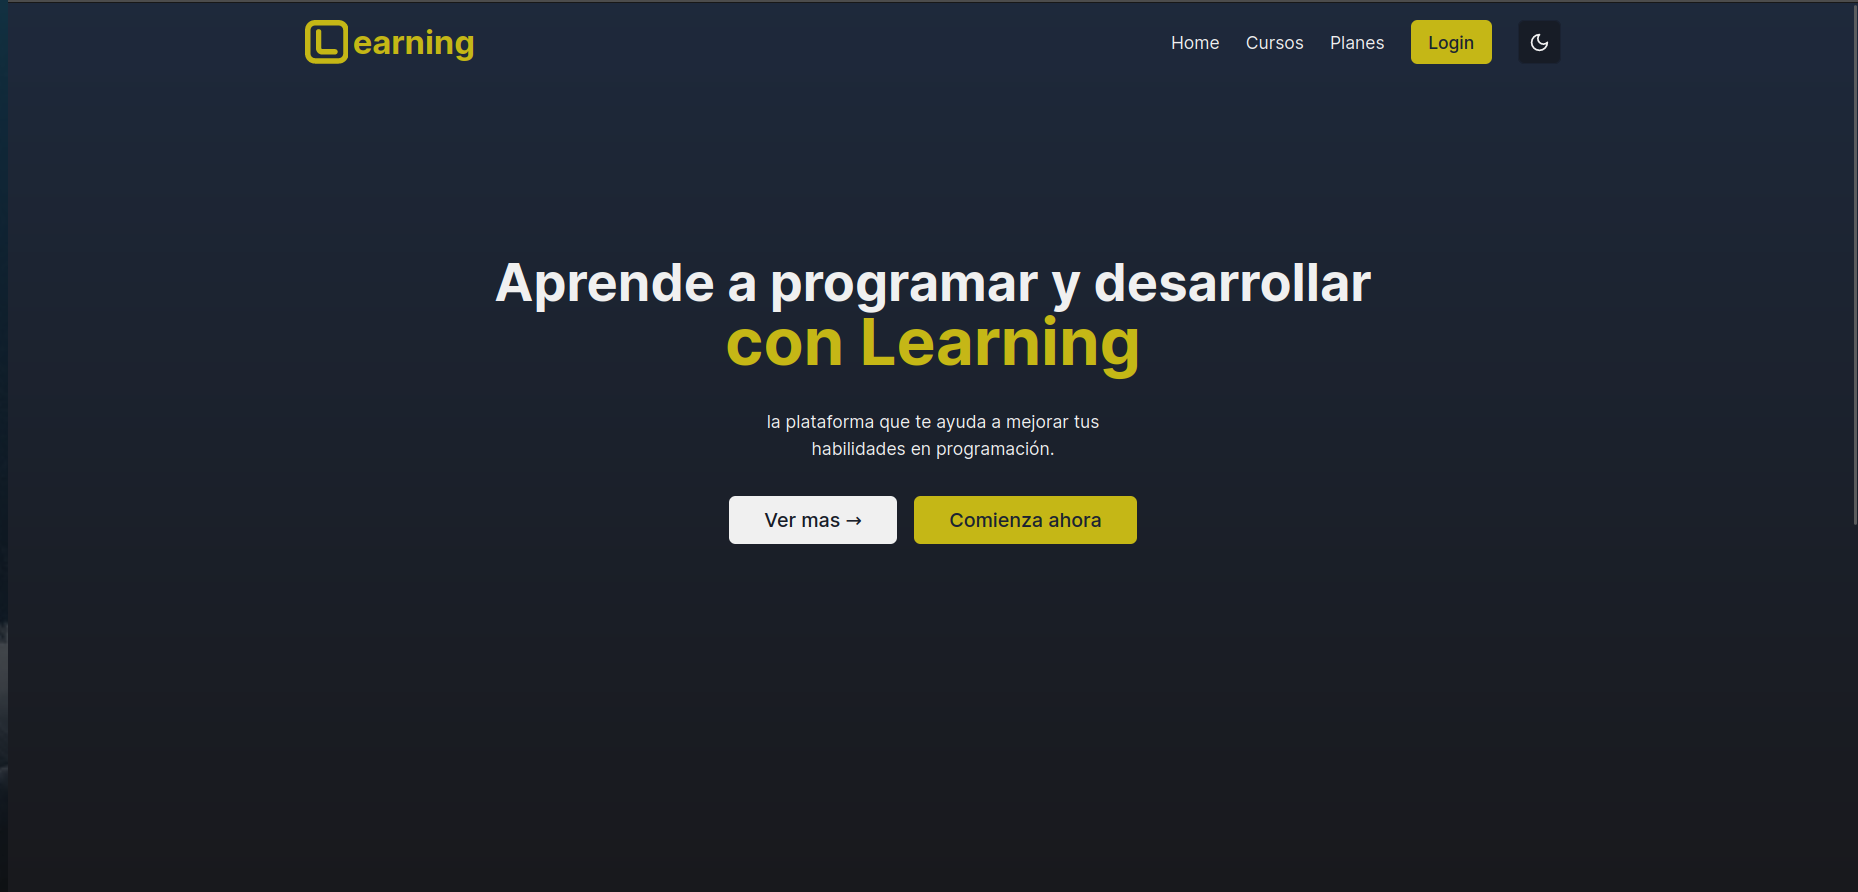
\includegraphics[width=1.0\textwidth]{img/H-DS.png}
    \caption{Home - Theme Dark and System}
  \end{figure}
  \begin{figure}[H]
    \centering
    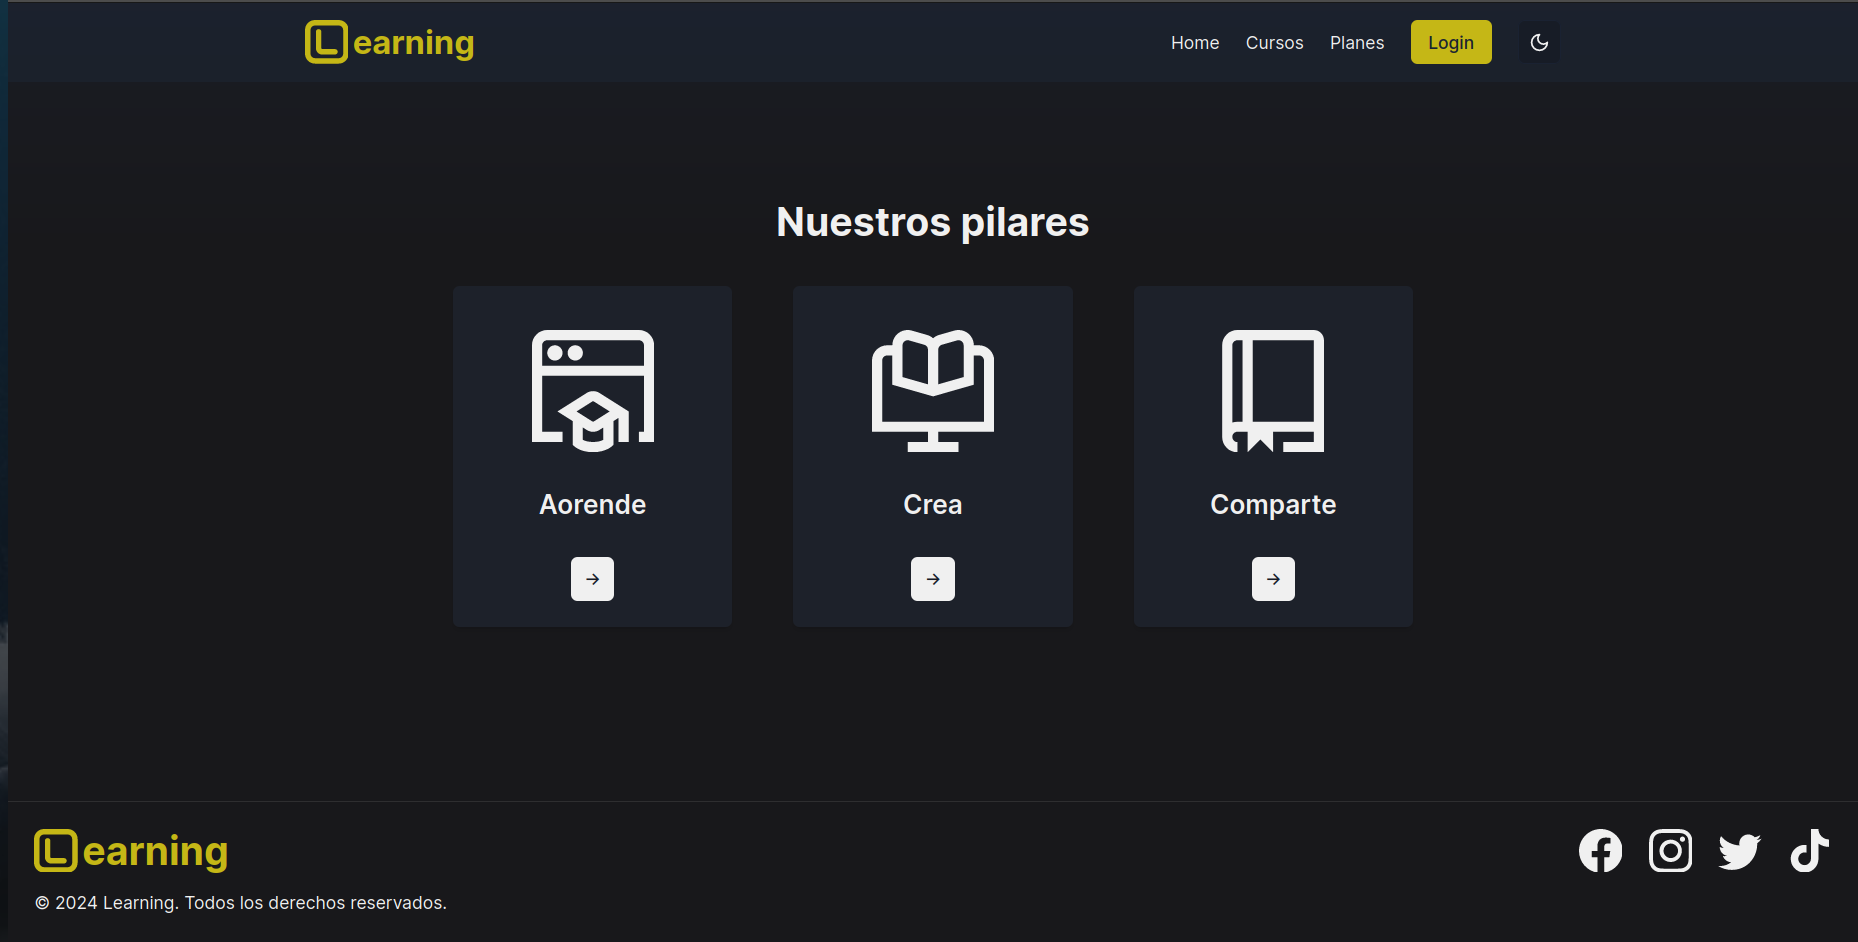
\includegraphics[width=1.0\textwidth]{img/H-DS2.png}
    \caption{Home - Theme Dark and System}
  \end{figure}
\subsection{Home - Theme Ligth}
  \begin{figure}[H]
    \centering
    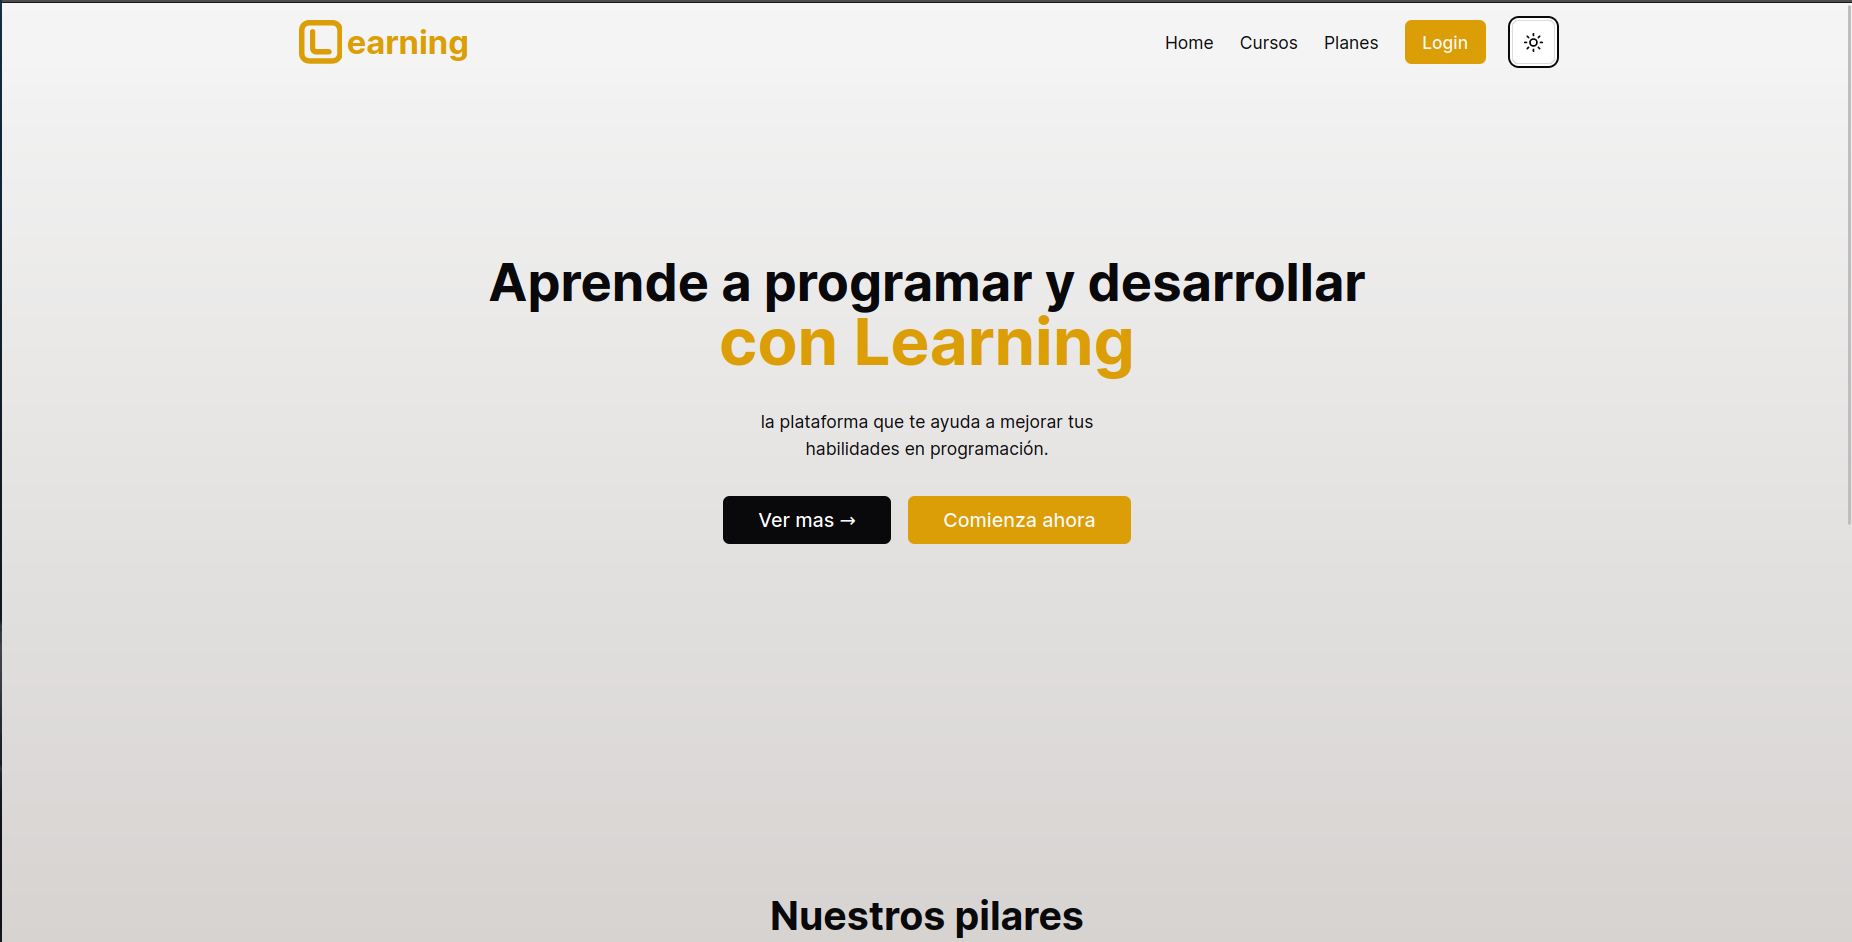
\includegraphics[width=1.0\textwidth]{img/H-L.png}
    \caption{Home - Theme Ligth}
  \end{figure}
  \begin{figure}[H]
    \centering
    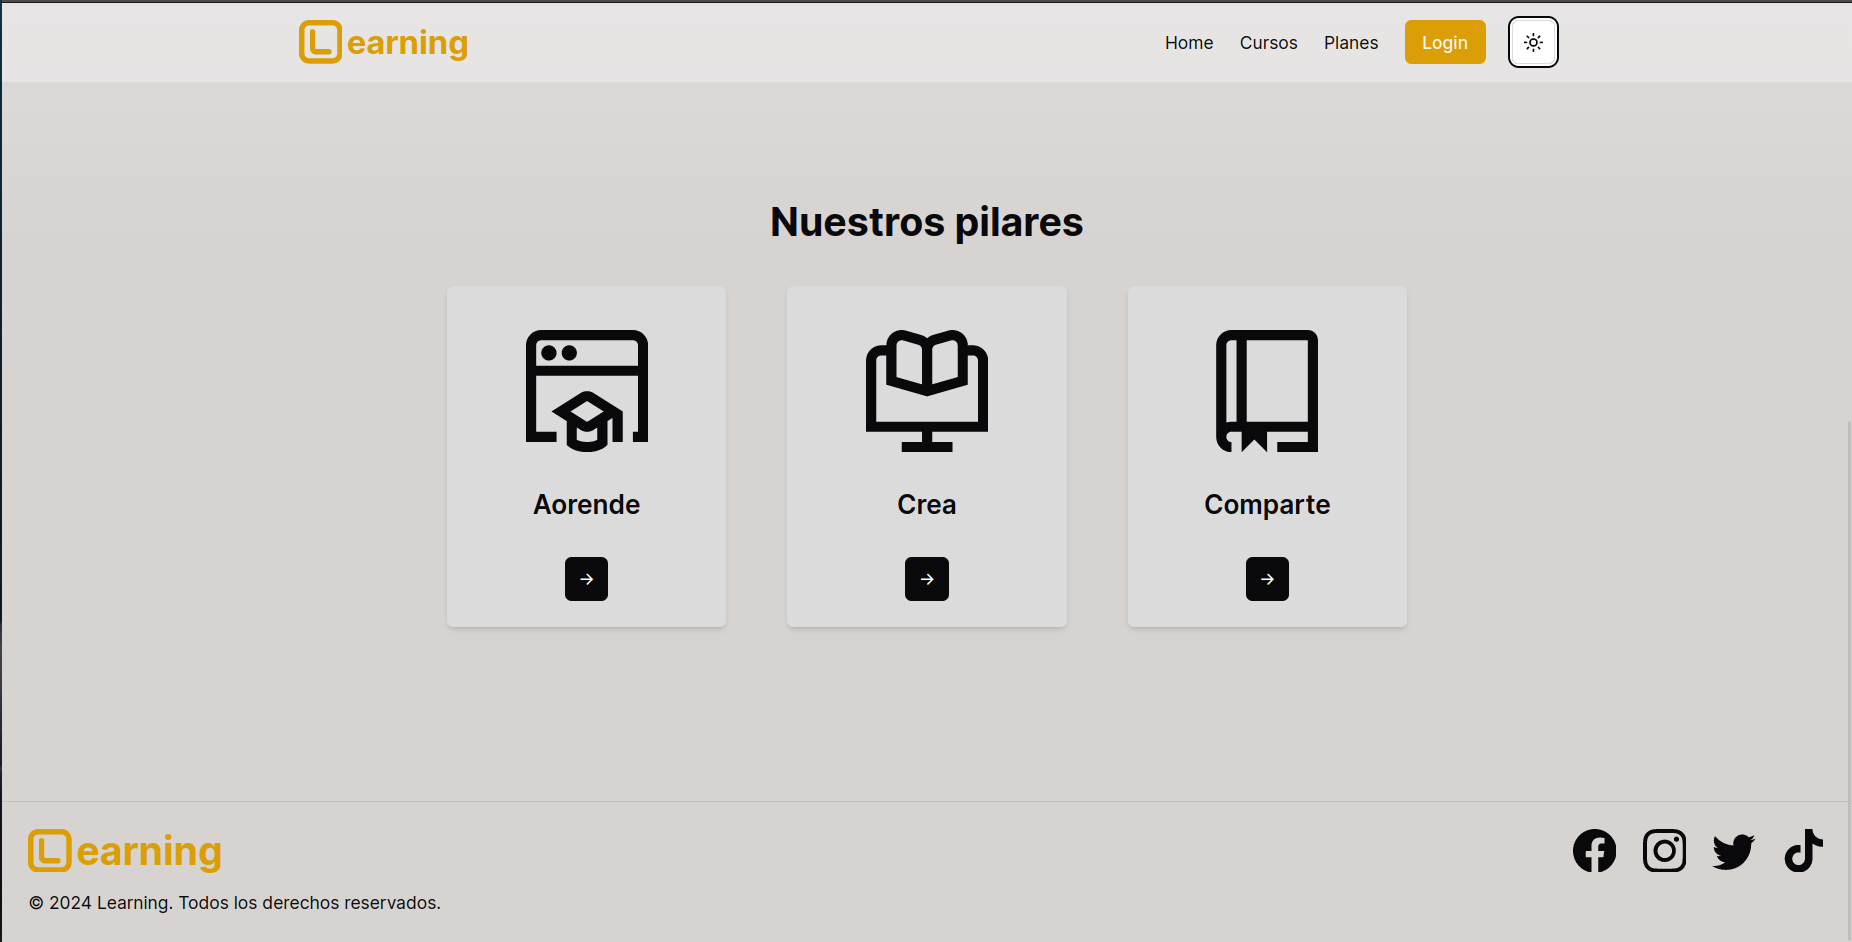
\includegraphics[width=1.0\textwidth]{img/H-L2.png}
    \caption{Home - Theme Ligth}
  \end{figure}
\subsection{Cursos - Theme Dark - System}
  \begin{figure}[H]
    \centering
    
\includegraphics[width=1.0\textwidth]{img/C-DS1.png}
    \caption{Cursos - Theme Dark and System}
  \end{figure}
  \begin{figure}[H]
    \centering
    
\includegraphics[width=1.0\textwidth]{img/C-DS2.png}
    \caption{Cursos - Theme Dark and System}
  \end{figure}
  \begin{figure}[H]
    \centering
    
\includegraphics[width=1.0\textwidth]{img/C-DS3.png}
    \caption{Cursos - Theme Dark and System}
  \end{figure}
  \begin{figure}[H]
    \centering
    
\includegraphics[width=1.0\textwidth]{img/C-DS4.png}
    \caption{Cursos - Theme Dark and System}
  \end{figure}
\subsection{Cursos - Theme Ligth}
  \begin{figure}[H]
    \centering
    
\includegraphics[width=1.0\textwidth]{img/C-L1.png}
    \caption{Cursos - Theme Ligth}
  \end{figure}
  \begin{figure}[H]
    \centering
    
\includegraphics[width=1.0\textwidth]{img/C-L2.png}
    \caption{Cursos - Theme Ligth}
  \end{figure}
  \begin{figure}[H]
    \centering
    
\includegraphics[width=1.0\textwidth]{img/C-L3.png}
    \caption{Cursos - Theme Ligth}
  \end{figure}
  \begin{figure}[H]
    \centering
    
\includegraphics[width=1.0\textwidth]{img/C-L4.png}
    \caption{Cursos - Theme Ligth}
  \end{figure}











\section{Frontend de la aplicación}
El directorio \texttt{client/} contiene el código fuente que está organizado de acuerdo al uso de \texttt{webpack}, un empaquetador de módulos JavaScript. Webpack es un paquete que se encarga de compilar múltiples archivos JavaScript, CSS y otros activos en un solo archivo o en varios archivos optimizados para la producción. Este paquete es utilizado por React, el framework más popular a nivel mundial para construir interfaces de usuario.

\subsection{tecnologías usadas}
\subsubsection{Framework React}
React es una biblioteca de JavaScript desarrollada por Facebook para construir interfaces de usuario. Se basa en componentes, lo que permite crear elementos de UI reutilizables y gestionables. Cada componente de React puede manejar su propio estado y lógica, y se puede combinar con otros componentes para crear aplicaciones complejas. 
\singlespacing
React también facilita la creación de aplicaciones web modernas con arquitecturas basadas en componentes, lo que permite a los desarrolladores dividir la UI en piezas más pequeñas y manejables. Esta modularidad no solo mejora la organización del código, sino que también facilita el mantenimiento y la escalabilidad del proyecto.

\paragraph{Ventajas de Usar React}
\begin{itemize}
  \item \textbf{Componentes Reutilizables}: Los componentes de React pueden ser reutilizados en diferentes partes de la aplicación, lo que reduce la duplicación de código y facilita el mantenimiento.
  \item \textbf{Virtual DOM}: Permite actualizaciones eficientes y rápidas del DOM, mejorando el rendimiento de la aplicación.
  \item \textbf{JSX}: Una extensión de JavaScript que permite escribir HTML dentro de JavaScript, haciendo que el código sea más legible y fácil de escribir.
  \item \textbf{Unidirectional Data Flow}: La gestión del estado en React es más predecible gracias al flujo de datos unidireccional, lo que facilita la depuración y el seguimiento de cómo los datos fluyen a través de la aplicación.
\end{itemize}

\paragraph{Estructura de un Componente React}
Cada componente en React puede definirse como una función o una clase que devuelve un fragmento de la interfaz de usuario. A continuación, se muestra un ejemplo de un componente funcional básico en React:

\begin{minted}{javascript}
import React from 'react';

function Welcome(props) {
  return <h1>Hello, {props.name}</h1>;
}

export default Welcome;
\end{minted}

En este ejemplo, \texttt{Welcome} es un componente funcional que toma \texttt{props} (propiedades) como argumento y retorna un encabezado con un saludo personalizado. Los componentes de clase también pueden definir métodos de ciclo de vida y manejar estados internos más complejos.

\subsection{Integración con Tailwind CSS}
Para estilizar los componentes de React, en este proyecto se utiliza Tailwind CSS. Tailwind es un framework de utilidades CSS que permite aplicar estilos directamente en los componentes mediante clases predefinidas. Esta metodología facilita el desarrollo de interfaces de usuario rápidas y consistentes.

El siguiente es un ejemplo de un componente estilizado con Tailwind CSS:

\begin{minted}{typescript}
import React from 'react';

function Button({ label }) {
  return (
    <button className="bg-blue-500 hover:bg-blue-700 text-white font-bold py-2 px-4 rounded">
      {label}
    </button>
  );
}

export default Button;
\end{minted}

En este ejemplo, las clases de Tailwind se utilizan para definir el estilo del botón, como el color de fondo, el comportamiento al pasar el ratón por encima, el color del texto y el espaciado.

\subsubsection{Webpack}
Webpack es una herramienta de construcción de módulos que se utiliza para agrupar, compilar y gestionar dependencias en proyectos JavaScript. Permite transformar archivos de diferentes tipos (JavaScript, CSS, imágenes, etc.) en un conjunto de activos que pueden ser servidos por un servidor web. Algunas características clave de Webpack incluyen:

\begin{itemize}
    \item \textbf{Entrada y Salida}: Webpack toma uno o varios archivos de entrada y los transforma en uno o varios archivos de salida optimizados.
    \item \textbf{Loaders}: Transforman archivos de otros tipos en módulos válidos que Webpack puede procesar.
    \item \textbf{Plugins}: Extienden la funcionalidad de Webpack para optimizar el empaquetado, gestionar el hot reloading, minificación, entre otros.
    \item \textbf{Code Splitting}: Permite dividir el código en diferentes archivos para optimizar el rendimiento y la carga inicial de la aplicación.
\end{itemize}

\subsubsection{Next.js}
Next.js es un framework para React que permite la creación de aplicaciones web tanto del lado del cliente como del servidor. Facilita la implementación de aplicaciones web con funcionalidades como el renderizado del lado del servidor (SSR), generación de sitios estáticos (SSG), y rutas dinámicas.

\begin{itemize}
    \item \textbf{Renderizado del Lado del Servidor (SSR)}: Permite generar contenido HTML en el servidor en lugar del cliente, lo que puede mejorar el rendimiento y SEO.
    \item \textbf{Generación de Sitios Estáticos (SSG)}: Genera páginas HTML estáticas en el momento de la compilación, optimizando el rendimiento y tiempo de carga.
    \item \textbf{Rutas Dinámicas}: Facilita la creación de rutas dinámicas basadas en la estructura de archivos del proyecto.
    \item \textbf{API Routes}: Permite definir endpoints API dentro del proyecto Next.js, facilitando la creación de backends ligeros.
\end{itemize}

Este directorio \texttt{client/} contiene una estructura definida y varios archivos de configuración esenciales para la correcta implementación de la aplicación.

\begin{itemize}
  \item \texttt{.eslintrc.json}: Configuración de ESLint para mantener la calidad y consistencia del código. A continuación se muestra un extracto relevante:
  \inputminted{json}{../client/.eslintrc.json}

  \item \texttt{tailwind.config.ts}: Configuración de Tailwind CSS para definir temas, colores, espaciados y otras utilidades personalizadas que se usarán en el proyecto:
  \inputminted{typescript}{../client/tailwind.config.ts}

  \item \texttt{postcss.config.mjs}: Configuración de PostCSS para transformar CSS con plugins, como \texttt{autoprefixer}:
  \inputminted{javascript}{../client/postcss.config.mjs}

  \item \texttt{tsconfig.json}: Configuración del compilador TypeScript para especificar opciones de compilación y manejo de archivos:
  \inputminted{json}{../client/tsconfig.json}

  \item \texttt{next.config.mjs}: Configuración específica de Next.js para definir rutas personalizadas, configuraciones de webpack y variables de entorno:
  \inputminted{javascript}{../client/next.config.mjs}

  \item \texttt{package.json}: Listado de dependencias y scripts del proyecto, incluyendo librerías y herramientas necesarias para el desarrollo y producción:
  \inputminted{json}{../client/package.json}

  \item \texttt{public/}: Contiene archivos estáticos como imágenes y fuentes que son servidos directamente por el servidor web.
\end{itemize}

\subsection{Autenticación con NextAuth}
NextAuth.js es una biblioteca completa para la autenticación en aplicaciones Next.js, soportando varios proveedores de autenticación. 

\subsubsection{Configuración de NextAuth}
La configuración se encuentra en \texttt{src/app/api/auth/[...nextauth]/authOptions.ts}. Este archivo define los proveedores de autenticación y los callbacks para manejar eventos durante el flujo de autenticación:
\inputminted{typescript}{../client/src/app/api/auth/\[...nextauth\]/authOptions.ts}

\subsubsection{Manejo de Rutas de Autenticación}
El endpoint de la API para autenticación está definido en \texttt{src/app/api/auth/[...nextauth]/route.ts}:
\inputminted{typescript}{../client/src/app/api/auth/\[...nextauth\]/route.ts}

\subsection{Lógica del Proyecto}
La lógica del proyecto se distribuye principalmente en el directorio \texttt{client/src/app/}, donde se define cómo se va a presentar el proyecto. 

\subsection{Estructura de Páginas y Componentes}
En este directorio, se organizan los componentes y páginas de la aplicación, excluyendo los que se encuentran en \texttt{client/src/components}, los cuales serán explicados a detalle porque son los components semilla que sirven de construcción para los componentes compuestos de este directorio.. Aquí se define la lógica de presentación y cómo interactúan los distintos componentes.

\section{Layout y Páginas}
El directorio \texttt{client/src/app/} contiene la estructura principal y las páginas de la aplicación. A continuación, se detallan los archivos más importantes.

\subsection{Layout Principal}
El archivo \texttt{layout.tsx} es el punto de entrada principal para la estructura del sitio. Define el layout global que se aplica a todas las páginas de la aplicación, proporcionando una consistencia en el diseño y la estructura.

\inputminted{typescript}{../client/src/app/layout.tsx}

En este archivo, se importa el archivo CSS global de Tailwind para aplicar los estilos a toda la aplicación. La estructura básica del layout incluye un componente \texttt{Header}, que puede contener elementos de navegación y logotipos, y un \texttt{main} que envuelve el contenido principal de cada página. El componente \texttt{children} representa el contenido dinámico que cambia según la página que se esté renderizando.
\singlespacing
El layout también puede incluir otros componentes comunes como el \texttt{Footer} y \texttt{Sidebar}, asegurando que todos los elementos de la UI compartidos se mantengan consistentes en toda la aplicación.

\subsection{Páginas y Rutas}
Cada página de la aplicación se define en un archivo separado dentro de \texttt{client/src/app/}. A continuación, se muestra un ejemplo de la página principal:

\inputminted{typescript}{../client/src/app/page.tsx}

En este archivo, la función principal exporta el contenido de la página, utilizando componentes de React para estructurar y estilizar la UI. En este caso, la página principal incluye un título y una descripción, junto con otros componentes que podrían estar presentes.

\subsection{Curso y Cursos}
Los directorios \texttt{curso} y \texttt{cursos} contienen archivos que definen las páginas y componentes específicos para manejar los cursos de la academia virtual. A continuación, se explica el contenido de estos directorios.

\subsubsection{Directorio \texttt{curso}}
El directorio \texttt{curso} contiene la estructura y lógica para mostrar información detallada de un curso específico. Esto incluye la descripción del curso, secciones, instructor y recursos adicionales.

\inputminted{typescript}{../client/src/app/[cursoID]/page.tsx}

Este archivo es una página dinámica que muestra información detallada de un curso basado en su \texttt{id}. Utiliza el hook \texttt{useRouter} de Next.js para obtener el \texttt{id} de la URL y fetch datos del curso correspondiente desde la API. Se muestran detalles como el título del curso, descripción, secciones y el instructor.

\subsubsection{Directorio \texttt{cursos}}
El directorio \texttt{cursos} contiene la estructura y lógica para manejar la lista de todos los cursos y puede incluir filtros, búsqueda y categorización de los cursos.

\textbf{page.tsx}:
\inputminted{typescript}{../client/src/app/cursos/page.tsx}

Este archivo muestra una lista de todos los cursos disponibles en la plataforma. Puede incluir filtros para buscar cursos por nombre, categoría o nivel de dificultad. Utiliza fetch para obtener los datos de los cursos desde la API y muestra cada curso en una tarjeta.
\singlespacing
Este archivo muestra los cursos filtrados por una categoría específica. Utiliza el hook \texttt{useRouter} de Next.js para obtener la categoría de la URL y fetch los cursos que pertenecen a esa categoría desde la API. Los cursos se muestran en tarjetas similares al archivo \texttt{index.tsx}.

\subsection{Fetch de Datos}
Aunque la funcionalidad de fetch aún no está implementada, veremos que su inclusión será para mejorar la interacción con el backend y la presentación dinámica de datos.



\end{document}
